\subsection{Estructuras para implementar \textsc{Disjoint-Set}}

Como parte del trabajo la cátedra requirió implementar el \textsc{Disjoint-Set}
con 3 estructuras distintas, las listamos en conjunto con la complejidad de las
operaciones antes descriptas:

\begin{itemize}
	\item Representado como arreglo de componentes
	\begin{itemize}
		\item \Call{Nuevo}{s}: $O(s)$
		\item \Call{Buscar}{ds, $e$}: $O(1)$
		\item \Call{Unir}{ds, $a$, $b$}: $O(n)$
		\item \Call{Tamaño}{ds, $e$}: $O(1)$
	\end{itemize}
	\item Representado como árbol
	\begin{itemize}
		\item \Call{Nuevo}{s}: $O(s)$
		\item \Call{Buscar}{ds, $e$}: $O(n)$
		\item \Call{Unir}{ds, $a$, $b$}: $O(1)$
		\item \Call{Tamaño}{ds, $e$}: $O(1)$
	\end{itemize}
	\item Representado como árbol con \emph{path compression}
	\begin{itemize}
		\item \Call{Nuevo}{s}: $O(s)$
		\item \Call{Buscar}{ds, $e$}: $O(\alpha(s))$
			\textbf{(amortizado)}
		\item \Call{Unir}{ds, $a$, $b$}: $O(\alpha(s))$
			\textbf{(amortizado)}
		\item \Call{Tamaño}{ds, $e$}: $O(\alpha(s))$
			\textbf{(amortizado)}
	\end{itemize}
\end{itemize}

Sumado a esto, las representaciones de árbol pueden elegir si unir por mayor
rango o por mayor tamaño (en nuestro caso particular implementamos por mayor
tamaño).

\subsubsection{Resultados con distintos tamaños de imagen}

En esta apartado Se quiere determinar el comportamiento de nuestros algoritmos propuestos con diferentes tamaños de imagen. Queremos verificar en cada uno de ellos como se mueve el timpo de ejecución. 

Para esto se usarán 3 imagenes con dimensiones cuadradas por su facilidad para redimensionarlas. Luego los candidatos se expondrán en formatos de $[100x100px,200x200px...700x700px]$,

\begin{figure}[H]
	\centering
	\begin{subfigure}{0.3\linewidth}
		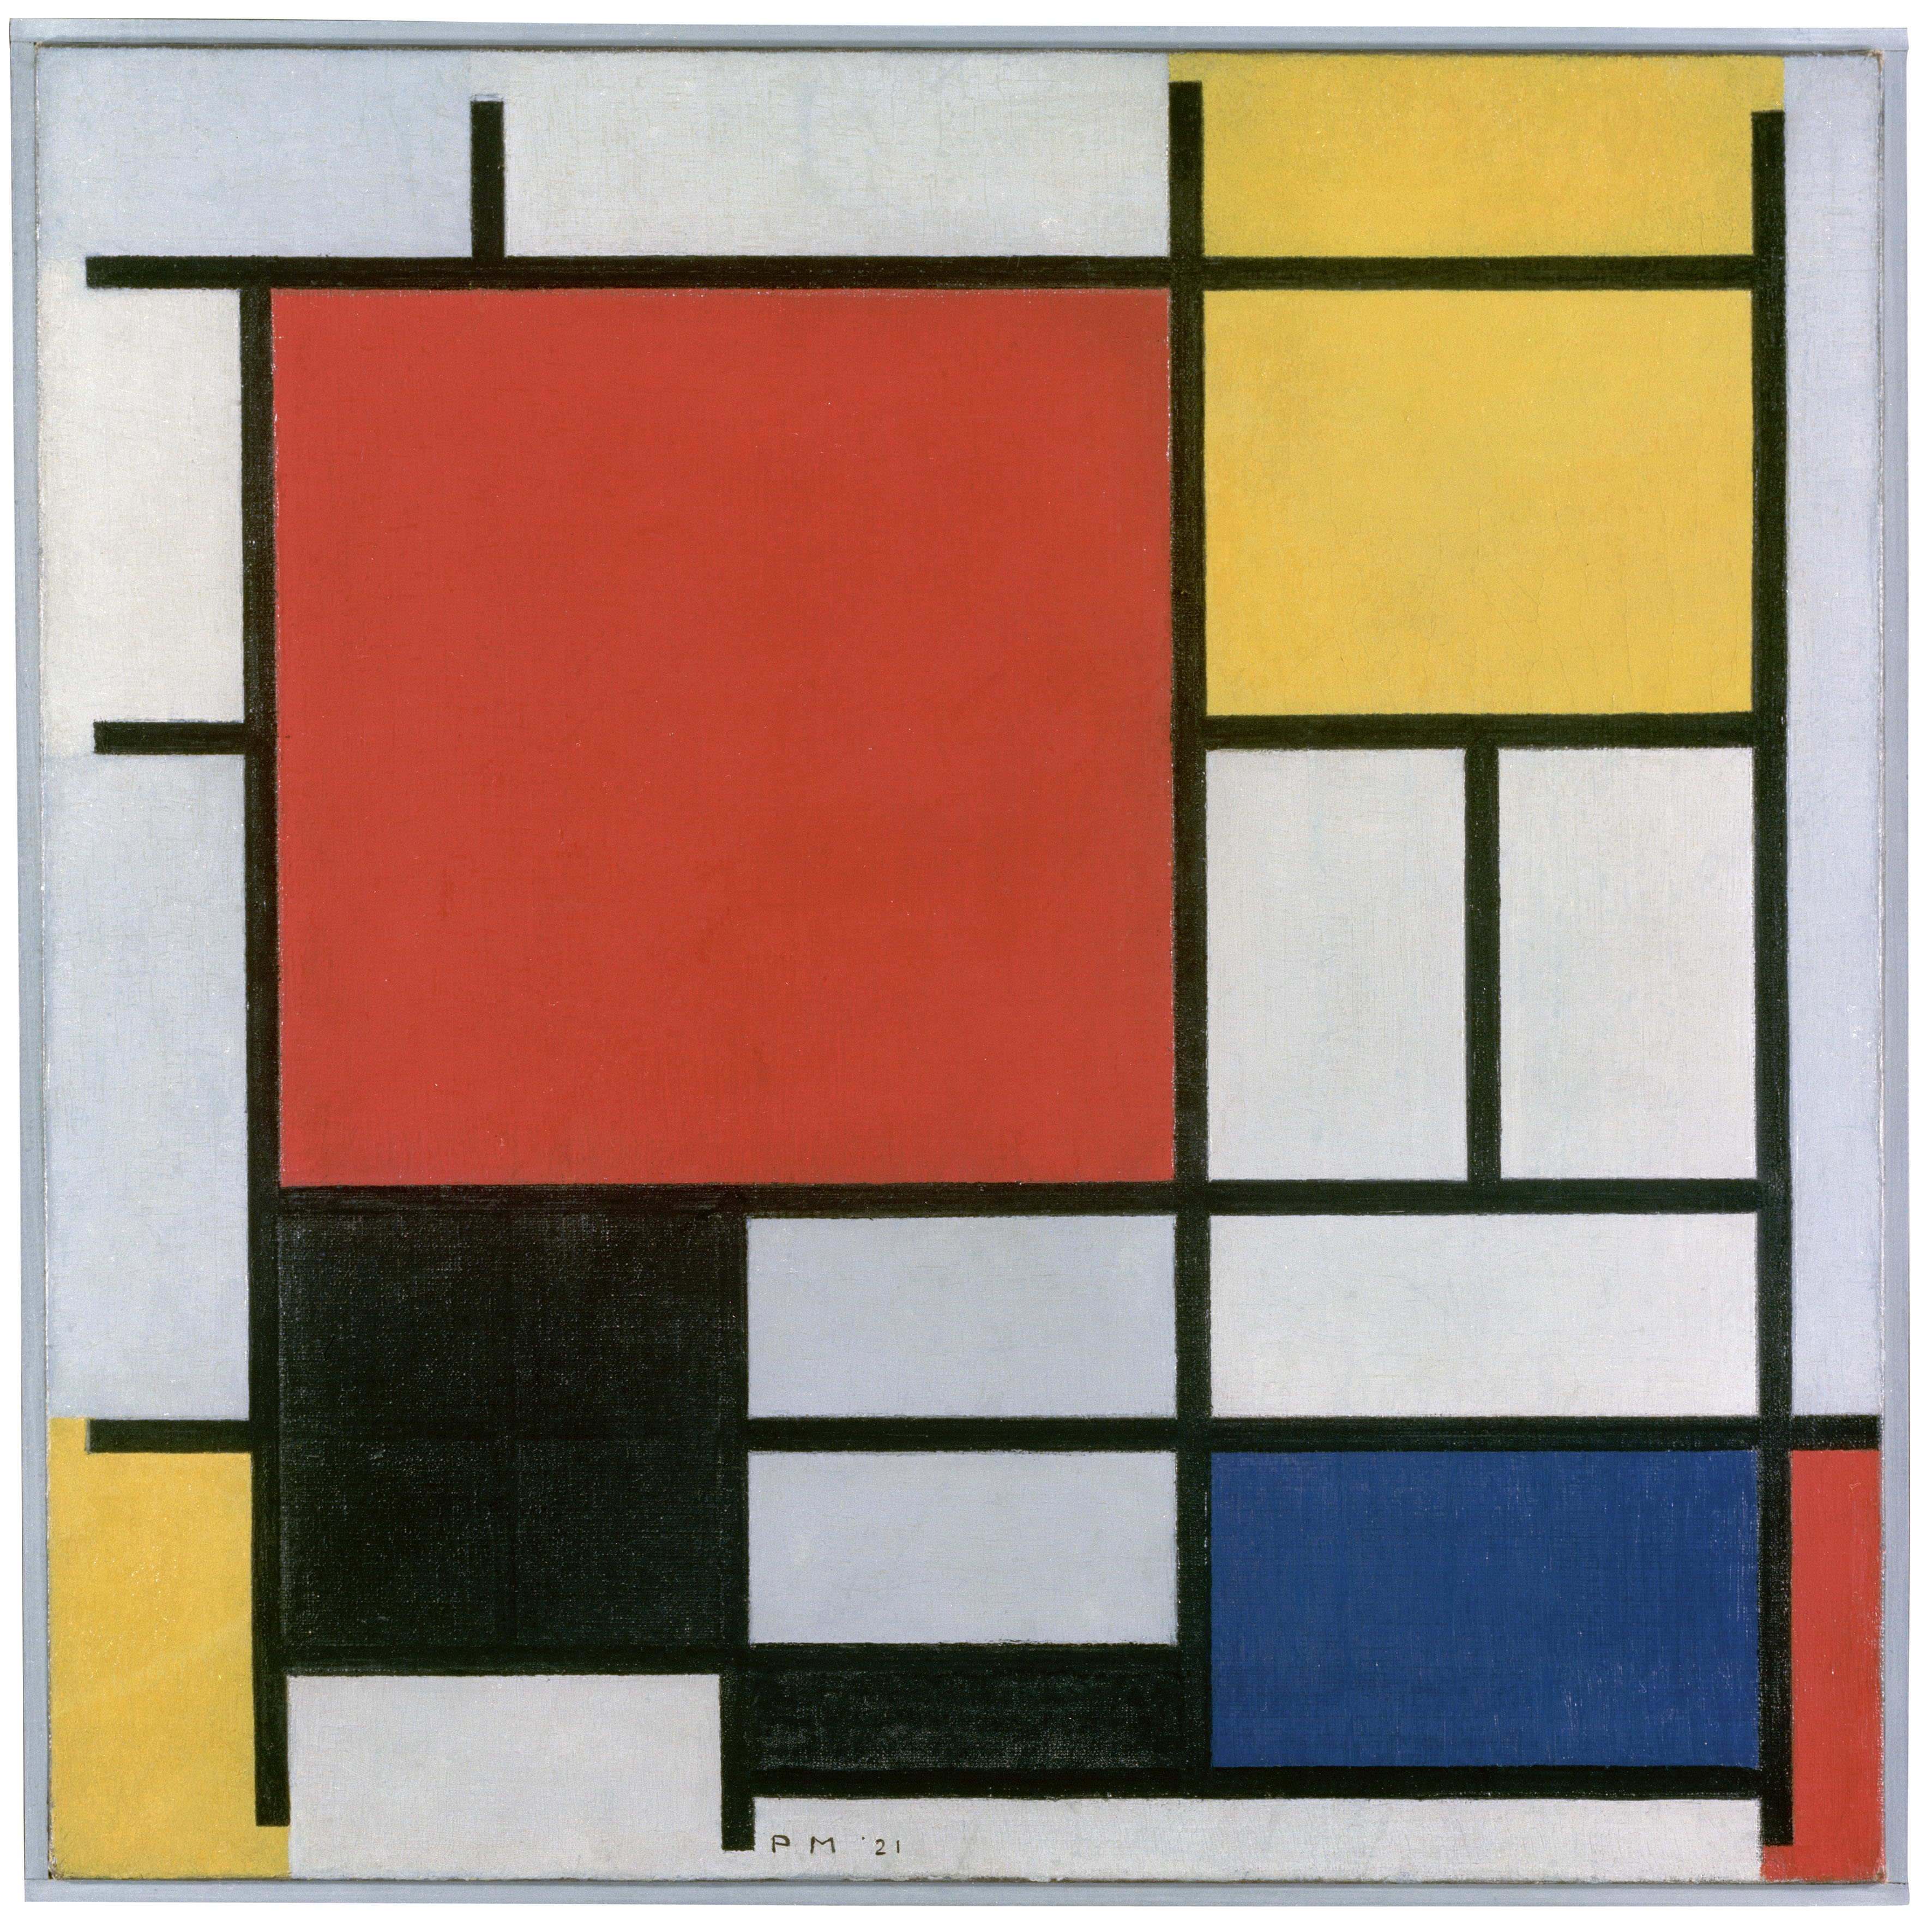
\includegraphics[width=\linewidth]{segmentation/entradas-posta/mondrian}
		\caption{Mondrian}
	\end{subfigure}
	\begin{subfigure}{0.3\linewidth}
	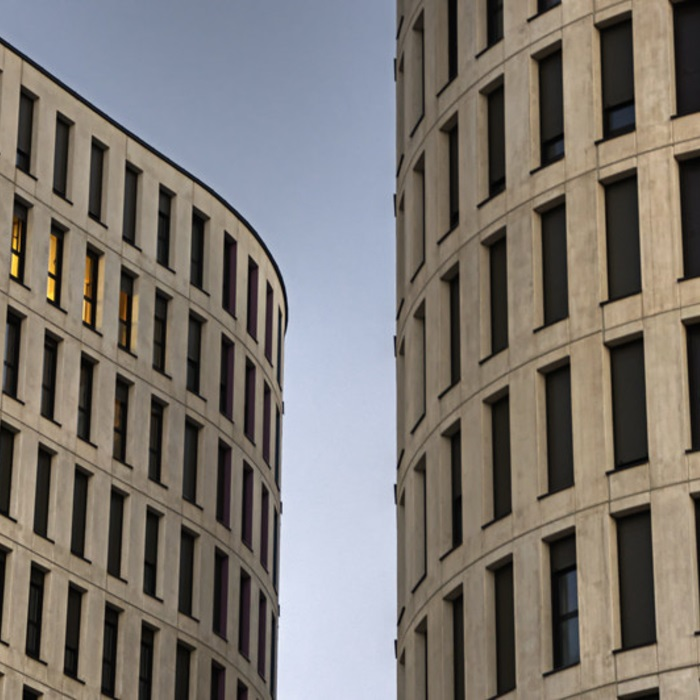
\includegraphics[width=\linewidth]{segmentation/entradas-posta/edificios}
	\caption{Edificios}
	\end{subfigure}
	\begin{subfigure}{0.3\linewidth}
		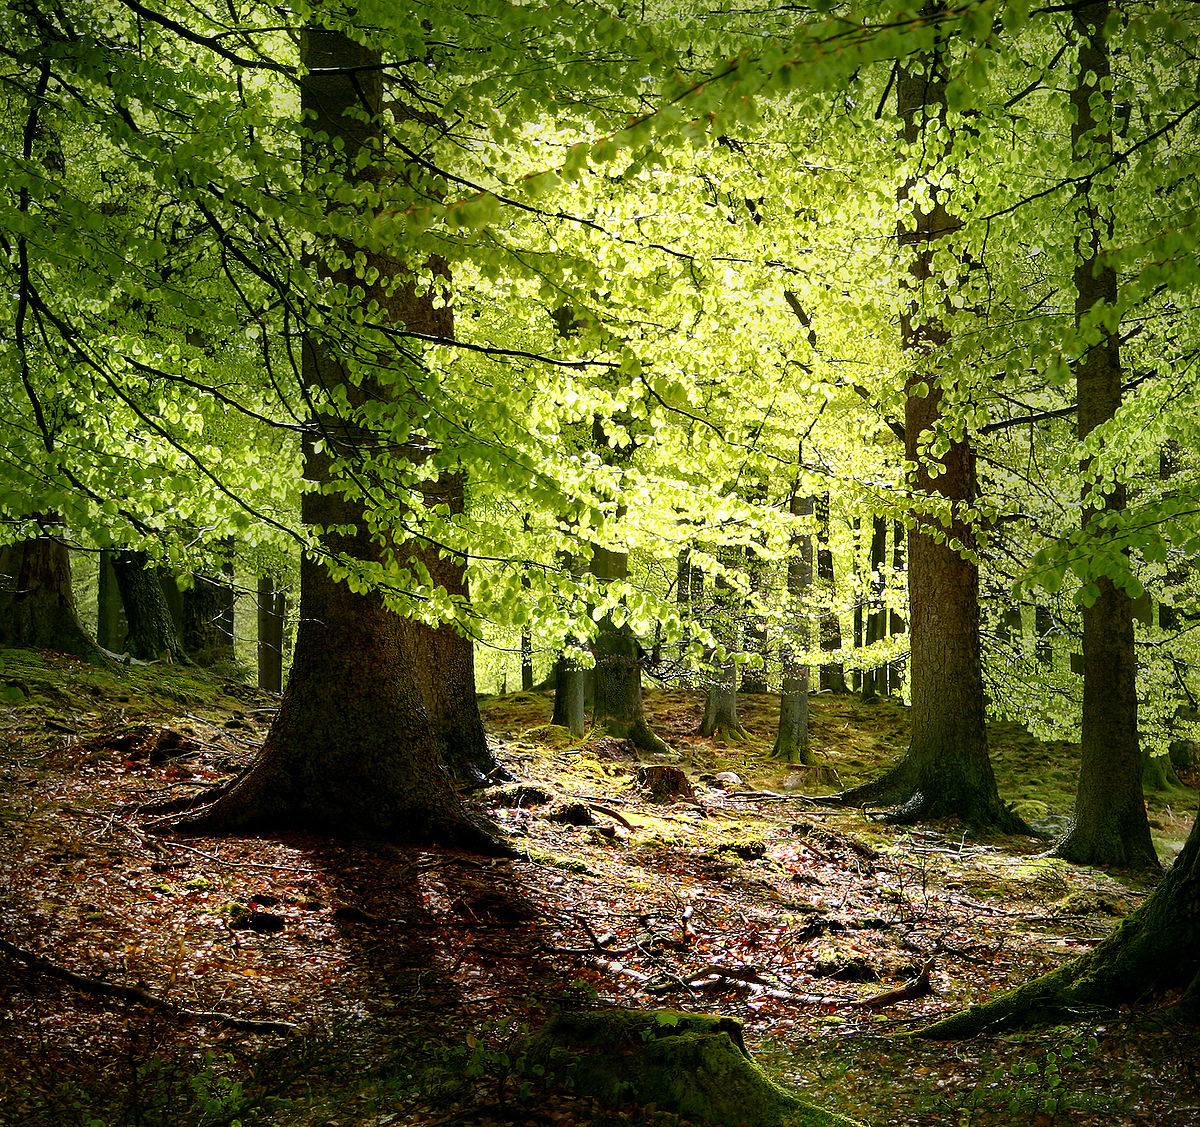
\includegraphics[width=\linewidth]{segmentation/entradas-posta/bosque}
		\caption{Bosque}
	\end{subfigure}
\end{figure}

Las 3 imagenes han sido seleccionadas para no compartir nada en común, así mismo se decidió que cada una de ellas posean diferentes dificultades de seccionamiento. Por ejemplo en la $Fig_A$ es trivial pensar cual sería la segmentación correcta.

Sin embargo en $Fig_B$ esto no es tan simple, sin embargo se podría definir un seccionamiento razonable por ejemplo seccionar el cielo de cada uno de los edificios y sus respectivas ventanas. En $Fig_C$ es muy dificil interpretar que se entiende por una segmentación \textit{"suficientemente buena"}

En cada una de las generaciones se setean $k = 300$, $\sigma = 0.8$, con $g$ deshabilitado. No nos interesa ver si la modificación de estos parámetros puede alterar los tiempos de ejcución. Dicha experimentación se vera en secciones posteriores.


\begin{figure}[H]
	\centering
	\includegraphics[width=0.75\linewidth]{segmentation/experimentacion/distintas-fotos-arreglo}
	\caption{Segmentación disjoint-set con arreglo.}
\end{figure}

\begin{figure}[H]
	\centering
	\includegraphics[width=0.75\linewidth]{segmentation/experimentacion/distintas-fotos-arbol}
	\caption{Segmentación disjoint-set con árbol.}
\end{figure}

\begin{figure}[H]
	\centering
	\includegraphics[width=0.75\linewidth]{segmentation/experimentacion/distintas-fotos-arbol-compr}
	\caption{Segmentación disjoint-set con árbol con compresión.}
\end{figure}

En los 3 algoritmos podemos observar que un comportamiento similar, siendo el algoritmo de àrbol de compresión el que muestra un rendimiento superior lo cual es esperable.

\subsubsection{Influencia de los parámetros}

Esta sección del informe analiza el rendimiento de las distintas
representaciones variando los parámetros $k$ y $g$\footnote{Valores de $\sigma$
mayores aumentarían el tiempo requerido de procesamiento pero ese procesamiento
se realiza antes de cualquier llamada a las estructuras que son relevantes a
esta sección del informe.}.

Dado que \textsc{Buscar} es considerablemente más simple en las
implementaciones con arreglo de componententes creemos que es esperable que
presente un rendimiento levemente superior para valores de $k$ y $g$ muy bajos
(dónde se realizan muy pocas llamadas a \textsc{Unir}).

Para realizar estos experimentos tomamos una sola imagen como entrada
(\texttt{autitos.jpg}) sobre la cuál experimentamos. La decisión de tomar una
única imagen fué debido a que queremos medir el efecto de los parámetros en una
imagen dónde estos tengan relevancia (en una imagen completamente plana variar
$k$ o $g$ no cambiaría la segmentación resultante, las llamadas a \textsc{Unir}
y \textsc{Buscar} serían siempre las mismas).

\begin{figure}[h]
	\centering
	\begin{subfigure}{0.4\linewidth}
		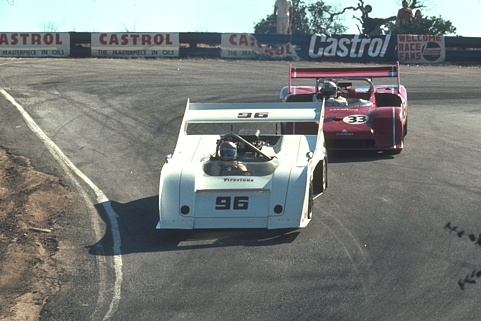
\includegraphics[width=\linewidth]{segmentation/entradas-posta/autitos}
		\caption{Entrada}
	\end{subfigure}
	\begin{subfigure}{0.4\linewidth}
		\includegraphics[width=\linewidth]{segmentation/salidas/{0.8.autitos.jpg.300.1000}.png}
		\caption{Segmentación}
	\end{subfigure}
	\caption{$\sigma = 0.8,\ k = 300,\ g = 1000$.}
\end{figure}

\subsubsection{Resultados variando $k$}

En el primer experimento decidimos medir el tiempo que tardaba el paso de
segmentación variando el $k$ de $0$ a $1200$ con incrementos de a $50$.

\begin{figure}[h]
	\centering
	\includegraphics[width=0.75\linewidth]{segmentation/experimentacion/variar-k}
	\caption{Tiempo incurrido por el proceso de segmentar al variar el $k$}
\end{figure}

Cuándo $k$ es $0$ el gráfico muestra que la segmentación realiza poco trabajo,
pero a partir de $50$ no muestra ninguna tendencia clara. Cómo la
experimentación se realizó con la misma entrada siempre esto da indicios de que
el coste de este trabajo no se ve influído más que por las características del
grafo grilla que se construye.

\subsubsection{Resultados variando $g$}

Dado que la granularidad varía su trabajo de acuerdo al $k$ elegido decidimos
tomar $k$ entre $0$ y $1200$ y variar el $g$ entre $1$ y $991$ en incrementos
de $10$.

\begin{figure}[h]
	\centering
	\includegraphics[width=0.75\linewidth]{segmentation/experimentacion/variar-g-arreglo}
	\caption{Tiempo incurrido por el proceso de simplificar al variar el $g$}
\end{figure}

Para $k=0$ vemos que cómo que el set resultante de la segmentación tenga
muchísimos conjuntos pequeños logra que el tiempo que requiera la
simplificación sea considerablemente mayor. También vemos que cada
implementación llega a un mínimo dado un $g$ suficientemente alto dónde el
costo de hacer las llamadas a \textsc{Tamaño} superan a las pocas llamadas a
\textsc{Unir} resultantes de los chequeos.

\begin{figure}[h]
	\centering
	\includegraphics[width=0.75\linewidth]{segmentation/experimentacion/variar-g-arbol}
	\caption{Tiempo incurrido por el proceso de simplificar al variar el $g$}
\end{figure}

Tomar el árbol como representación el caso de $k=0$ arroja resultados
interesantes. Dado que no se comprime el árbol cuanto menos se unifiquen las
componentes menor es el coste de \textsc{Tamaño} que internamente realiza una
llamada a \textsc{Buscar}. Lamentablemente cómo no experimentamos con mayor
finura en los valores de $k$ entre $1$ y $150$ no podemos decir nada sobre cuál
sea la tendencia que toma el gráfico en ese rango, sí vemos una tendencia más
clara para el resto de los valores que tenemos información.

\clearpage

\begin{figure}[h]
	\centering
	\includegraphics[width=0.75\linewidth]{segmentation/experimentacion/variar-g-arbol-compr}
	\caption{Tiempo incurrido por el proceso de simplificar al variar el $g$}
\end{figure}

Finalmente, en la simplificación usando la representación de árbol con
compresión volvemos a ver las tendencias de la representación de arreglo pero
con tiempos la mitad de grandes. Dado que los costes teóricos deberían ser
diferentes pero vemos tendencias muy similares esto nos da indicios de que
nuestro experimento no supo elegir valores que evidencien esas
diferencias\footnote{O que nuestras implementaciones tienen errores que hacen
que no funcionen de la forma esperada.}
